\documentclass{article}
\usepackage[letterpaper, margin = 1in]{geometry}
\usepackage{graphicx}
\graphicspath{.}
\usepackage{float}
\usepackage{tabto}

\begin{document}

\noindent \textbf{Compressibility Effects} \\ \\ 
With the previous simulations showcasing the effects of changes in airfoil geometry to the lift spectrum, it is now of interest to understand the effects of compressibility to the current method. The first step in validating the code is the check the compressibility effects on a flat plate. The Prandtl-Glauret Transformation was applied to the BEM code in order to simulate compressibility effects. \\

\noindent As stated by the transform, it is desired that a 2D compressible plane (x,y) be transformed to an equivalent incompressible flow plane ($\epsilon, \eta$). The calculations can be then performed in the transformed incompressibility plane and then transformed back to the compressible plane in order to obtain required parameter data such as $c_L$ and $c_p$. The typical formulation used is shown below:
$$
\beta^2 \phi_{xx} + \phi_{yy} = 0  \qquad \qquad \beta = \sqrt{1-M_{\infty}^2} 
$$
$$
\epsilon = x   \quad \quad  \eta = \beta y \newline
$$
$$
c_p = \frac{c_{p_{o}}}{\beta} \newline  \qquad \qquad
c_L = \frac{c_{L_{o}}}{\beta} \newline
$$

\noindent The first case being considered is a flat plate with a freestream mach number of $M_{\infty}$ = 0.2. In order to validate the current method, the results will be compared to the Possio Code developed by "...." This code produces blade vortex interaction response of a flat plate for compressible cases. The figure below shows a comparison of the BEM code with compressibility modifications made, and the Possio code. The various lines on the graphs show the result of the BEM code for different discretization models. As can be seen from the figure, the linear discretization best matches with the results from the Possio code. 

\begin{figure}[h]
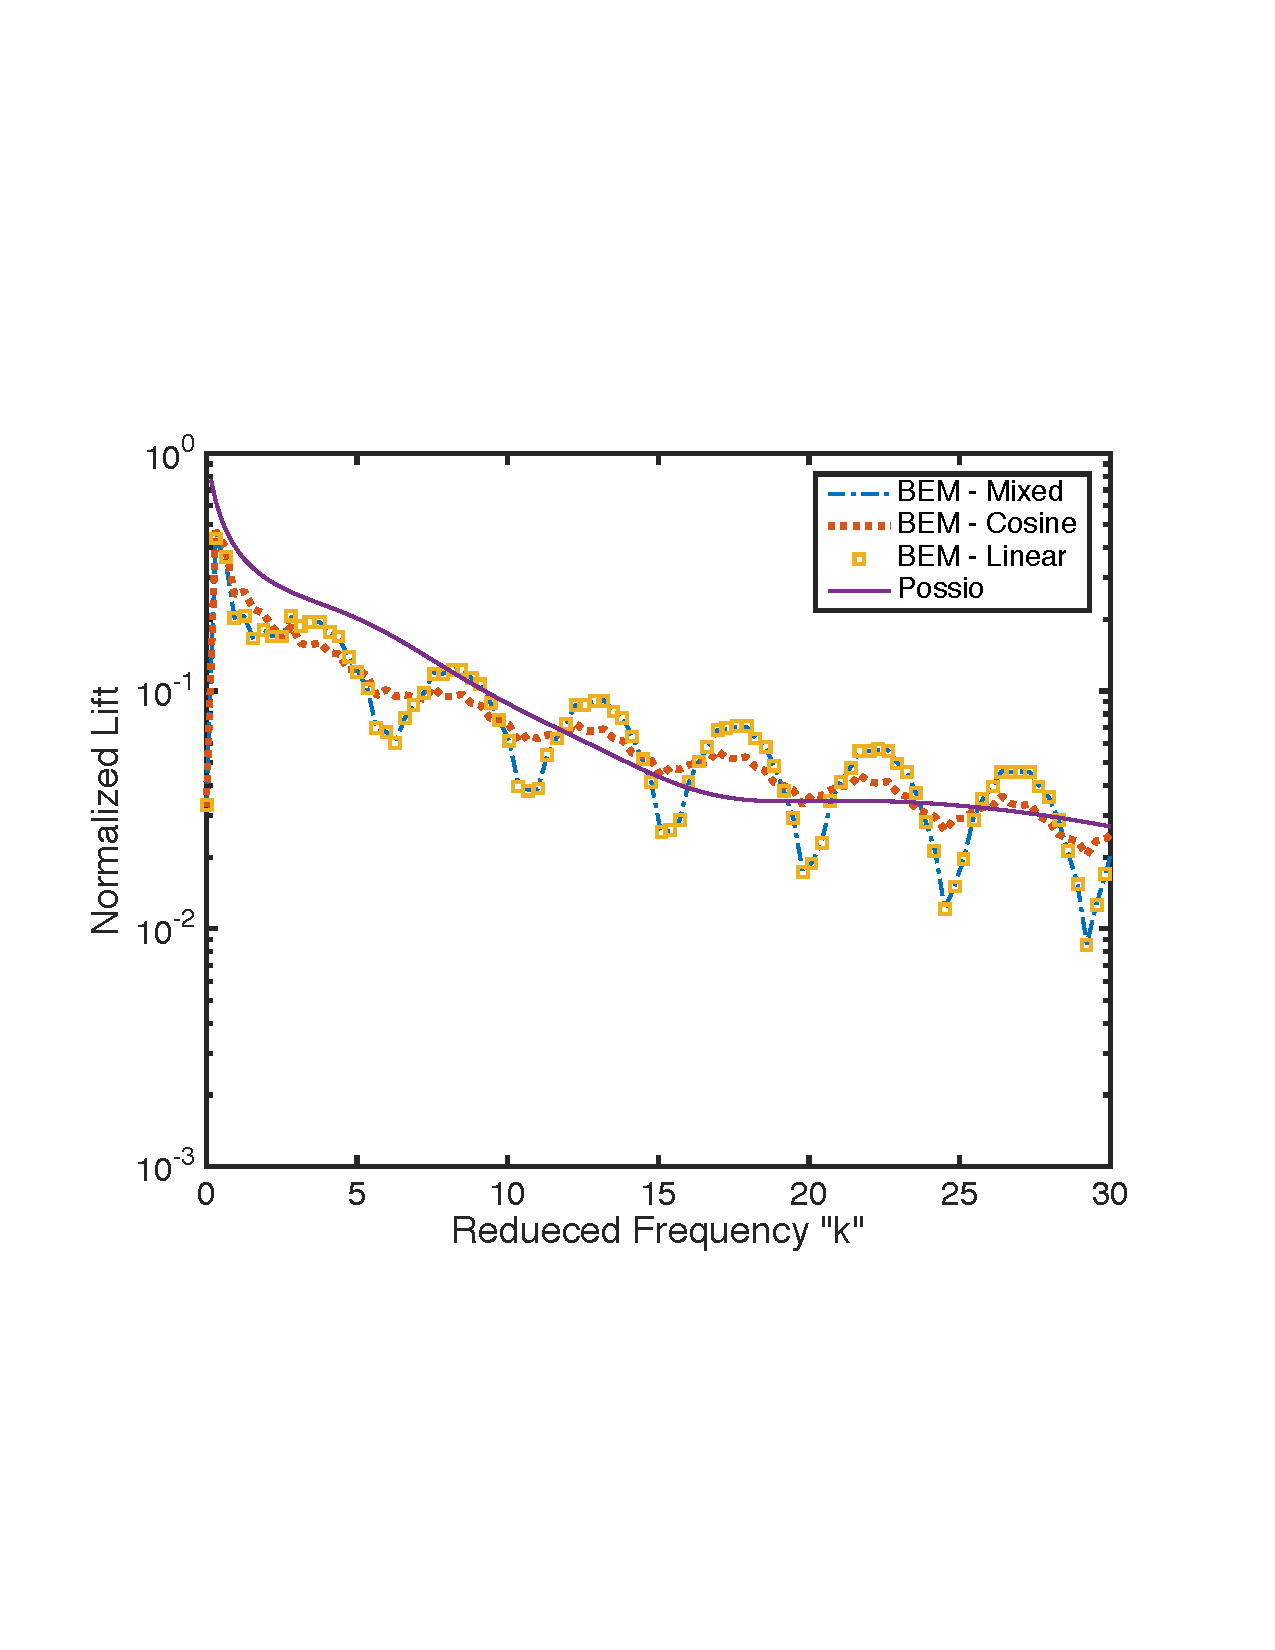
\includegraphics[ width = 4 in, height = 3 in]{BEM_Possio_Compare}
\centering
\caption{Comparison of discretizations of BEM results to Possio code results}
\end{figure}


\newpage
\noindent Using the linear discretization, the simulation was run for several mach numbers ranging from $M_{\infty}$ = 0.2 to  $M_{\infty}$ = 0.6. The figure below shows the response of the flat plate to the imposed vortex for the aforementioned mach numbers compared to the flat plate run results obtained from Possio.

\begin{figure}[h]
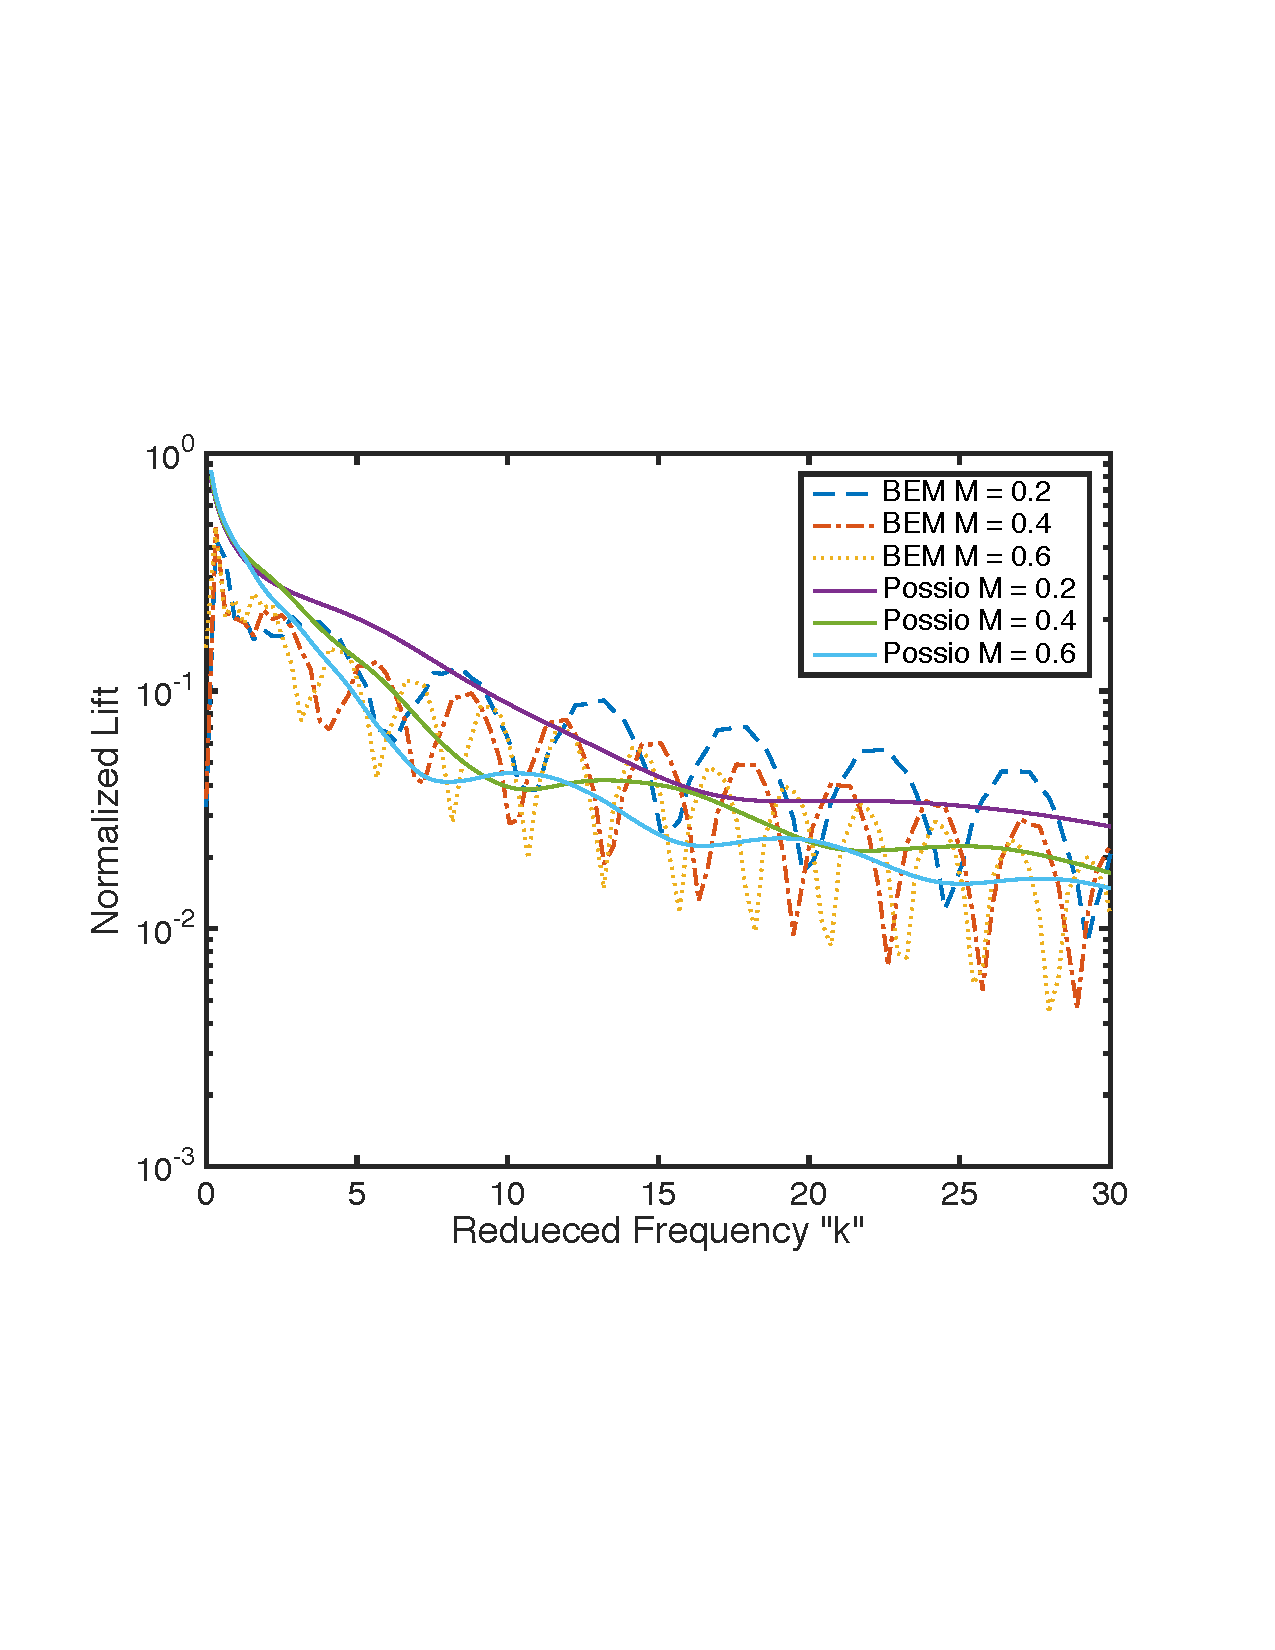
\includegraphics[width = 4 in, height = 3 in]{MachSweep_Compare}
\centering
\caption{BEM Code Results for Various Mach numbers compare to Possio}
\end{figure}






\end{document}
